\section{Le matériel expérimental}

\subsection{Scintillateurs}

Un scintillateur est un matériau dans lequel se produit un phénomène de scintillation suite à l'absorption de radiations ionisantes. Lorsqu'une particule traverse le scintillateur, celui-ci absorbe sont énergie et la ré-émet ensuite sous forme de lumière. Les scintillateurs présents dans vos dispositifs sont couplés à des photomultiplicateurs afin d'obtenir un détecteur à scintillation. \\

\begin{figure}[!h]
    \centering
	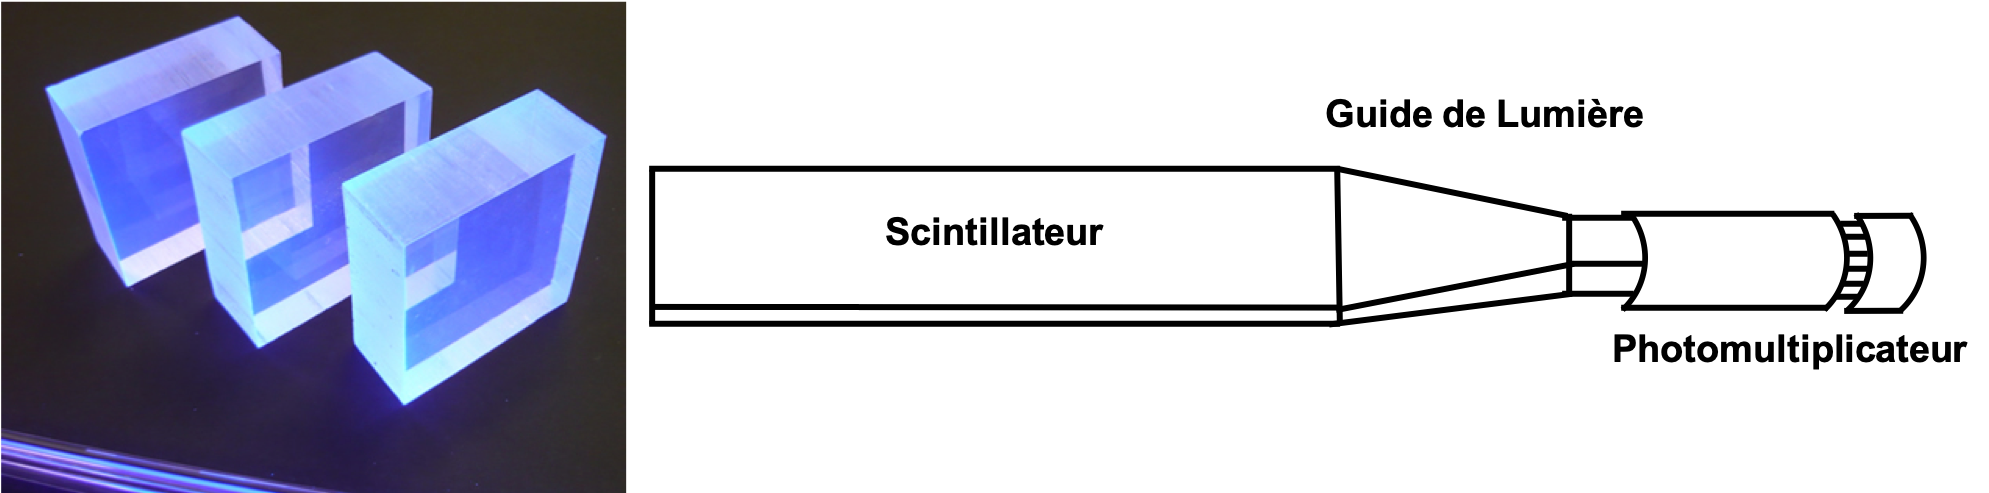
\includegraphics[width=\textwidth]{figures/Scintillateur.png}
    \caption{Schema d'un détecteur à scintillation.}
    \label{fig:PMT_readout} 
\end{figure}

\subsection{Photomultiplicateurs}

Les photmultiplicateurs (PMs) sont des détecteurs basés sur l'effet photoélectrique. Lorsqu'un photon arrive à la photocathode, il lui arrache un électron par effet photoélectrique. Le faible courant ainsi produit est ensuite amplifié par une série de dynodes afin d'obtenir un gain important. \\

\begin{figure}[!h]
    \centering
	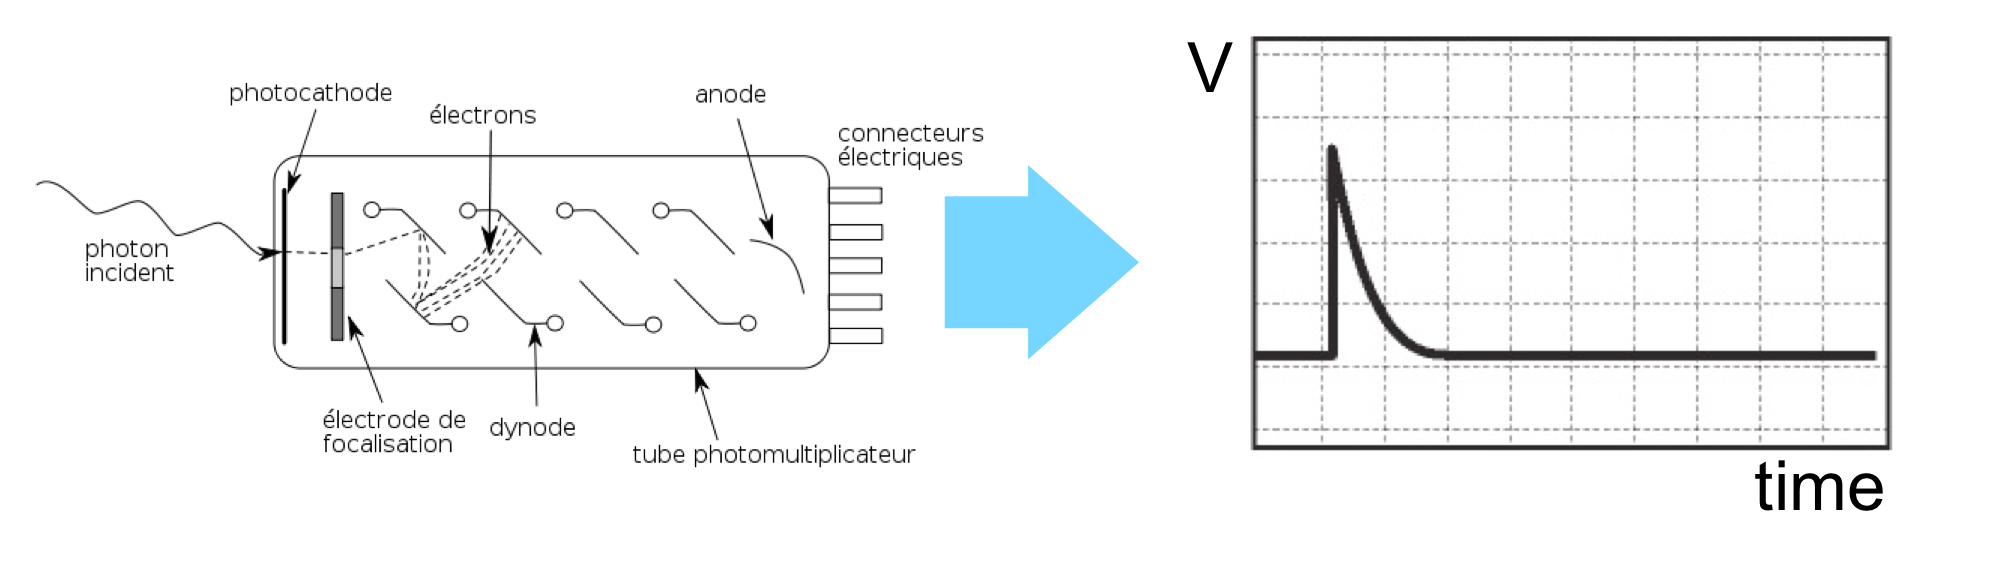
\includegraphics[width=\textwidth]{figures/PMT_readout.png}
    \caption{Schema du fonctionnement d'un photomultiplicateur(PMT).}
    \label{fig:PMT_readout} 
\end{figure}

Le gain du photomultiplicateur est défini comme :

\begin{equation}
G = \frac{Q_{1pe}}{q_{e}} 
\end{equation}

où $Q_{1pe}$ est la charge du premier photo-électron (pe) et $q_{e}$ représente la charge d'un électron. La résolution du photomultiplicateur est donnée par :

\begin{equation}
\sigma_{G} =  \frac{\sigma_{1pe}}{Q_{1pe}} * 100
\end{equation}

où $\sigma_{1pe}$ est l'écart-type du pic du premier pe.\\

Nous allons à présent étudier les différentes composantes d'un spectre en charge typique de la réponse d'un photomultiplicateur.\\

\begin{figure}[!h]
    \center{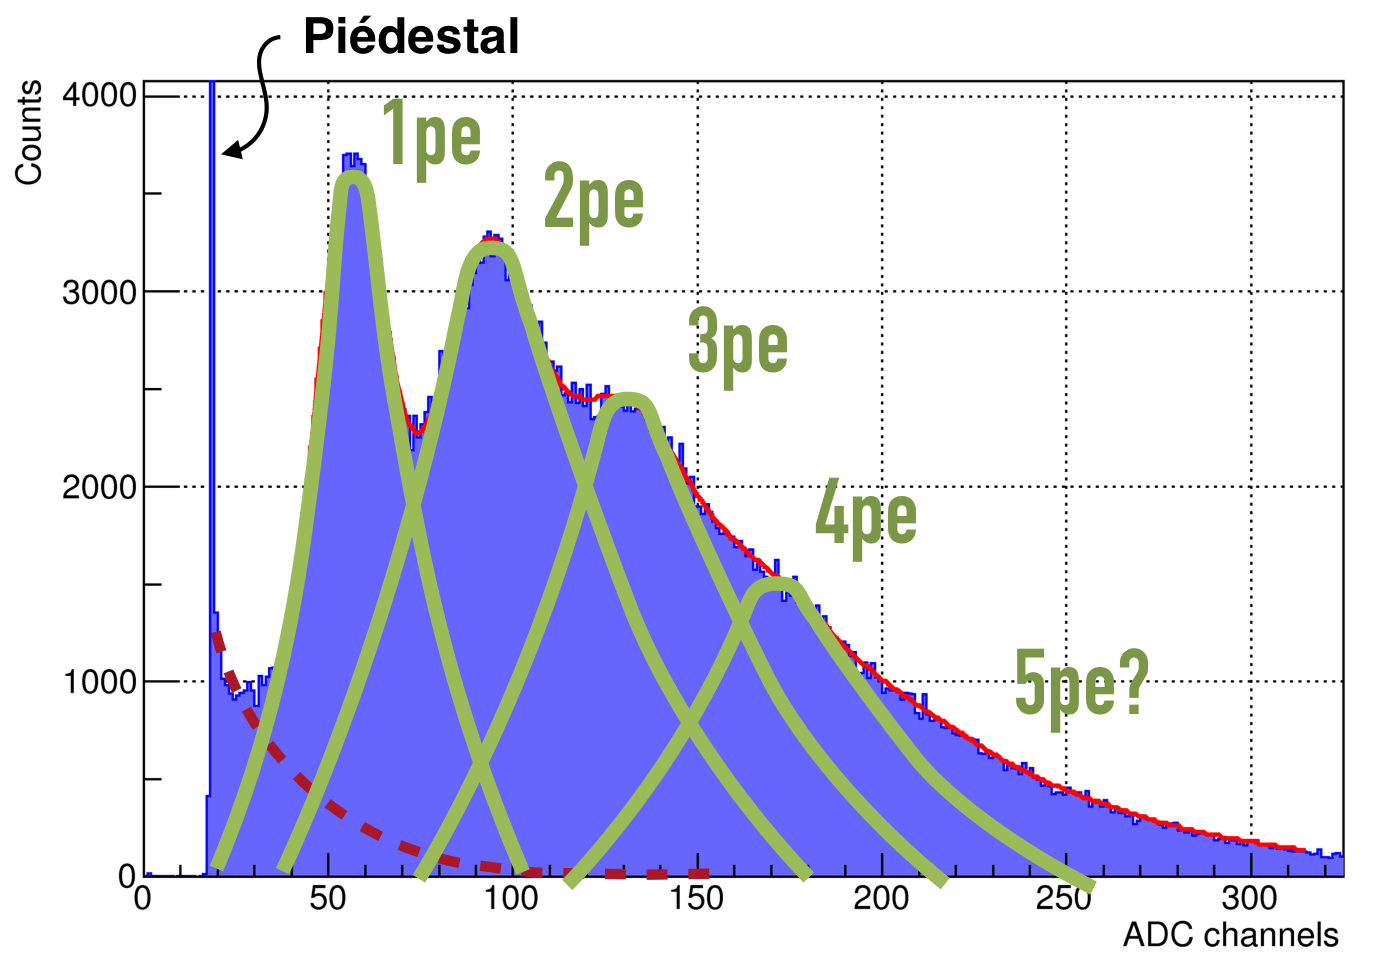
\includegraphics[width=0.7\textwidth]
    {figures/SpectreEnCharge.png}}
    \caption{\label{fig:spectre} Spectre en charge d'un photomultiplicateur.}
\end{figure}

\textbf{Piédestal :} Il s'agit d'évènements sans charge qui prennent la forme d'un pic en zéro. Afin de se débarrasser de cet effet, il vous faudra régler au mieux votre seuil.\\

\textbf{Dark current :} Il s'agit de bruit associé au PM, il survient lorsqu'un électron est arraché à une dynode sans qu'un photon incident n'arrive à la photocathode. Il nous donne une exponentielle décroissante. Cet effet est exacerbé lorsque la tension aux bornes du photomultiplicateur est élevée. \\

\textbf{Pic des photo-électrons :} Ce sont le réponse en charge du PM pour différent nombre de photo-électrons.\\

Le largeur de la gaussienne du premier photo-électron (1pe) va nous donner la résolution en charge du PM. La relation entre la hauteur des gaussiennes nous est donné par la distribution de Poisson.

\subsection{Aquisition de donn{\'e}es}

Nous allons à présent passer une revue les différents modules utilisés pour la prise de données. \\

\textbf{Alimentation} [figure \ref{fig:HV}] :\\
Les modules d'alimentations haute-tension permettent de contrôler la tension appliquées aux PMs et à l''OM.\\

\textbf{Scaler} [figure \ref{fig:scaler1}] :\\
Cette unité permet de compter les impulsions logiques entrantes. Le module de mesure standard CAMAC possède 12 entrées indépendantes. Il existe également des modules NIM possédant la même fonction. Ces derniers fonctionne sans acquisition de données et permettent de lire directement les résultats sur un écran intégré.\\


\begin{figure}[!h]
    \centering
    \begin{subfigure}[t]{0.2\textwidth}
        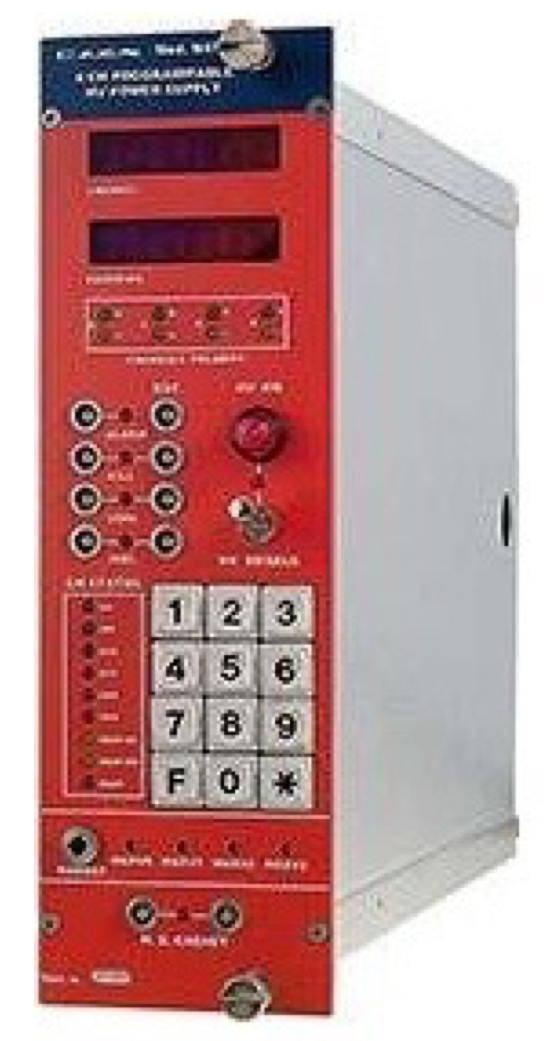
\includegraphics[height=0.25\textheight, width=\textwidth, keepaspectratio]{figures/Alim1.png}
        \caption{Alimentation de haute tension}
        \label{fig:HV}
    \end{subfigure}
    \hfill
    \begin{subfigure}[t]{0.2\textwidth}
        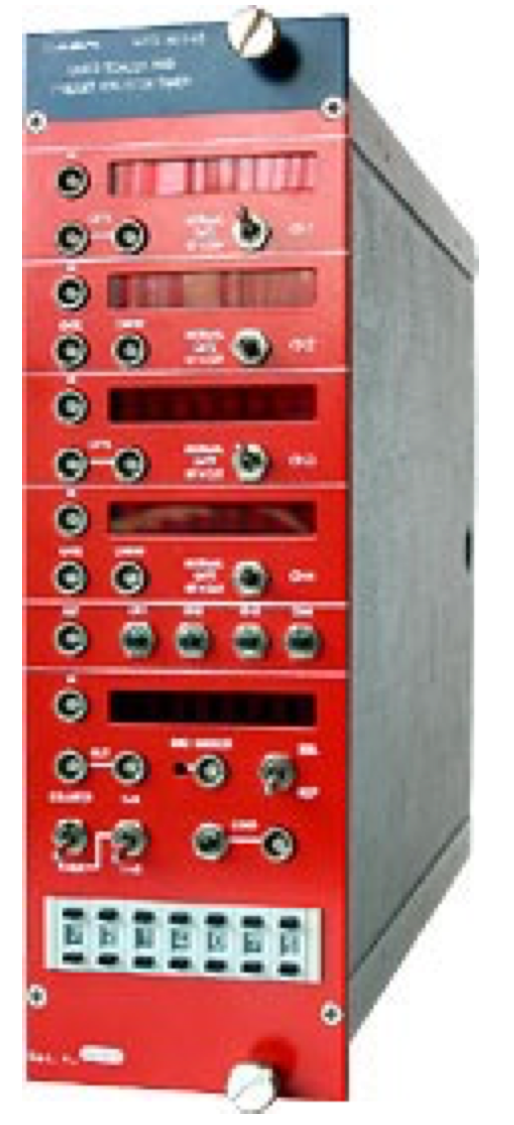
\includegraphics[height=0.25\textheight, width=\textwidth, keepaspectratio]{figures/scaler.png}
        \caption{Scaler NIM}
        \label{fig:scaler1}
    \end{subfigure}
    \hfill
    \begin{subfigure}[t]{0.2\textwidth}
        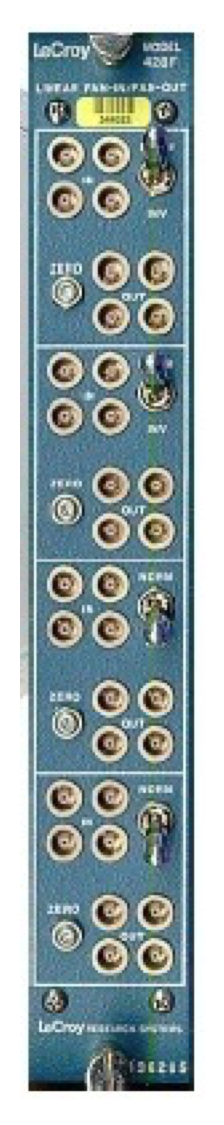
\includegraphics[height=0.25\textheight, width=\textwidth, keepaspectratio]{figures/FanInFanOut.png}
        \caption{Distributeur de signal \emph{fan-in-fan-out}}
        \label{fig:fifo}
    \end{subfigure}
    \hfill
    \begin{subfigure}[t]{0.2\textwidth}
        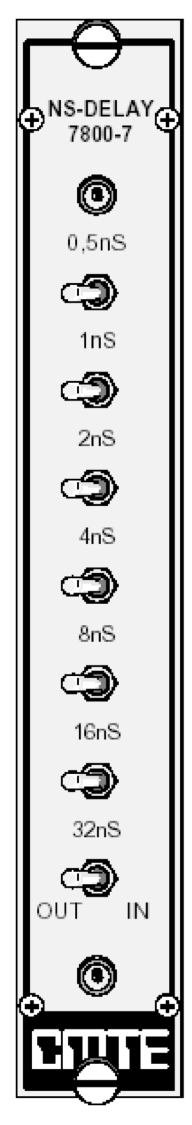
\includegraphics[height=0.25\textheight, width=\textwidth, keepaspectratio]{figures/delay.png}
        \caption{Delayeur de signal}
        \label{fig:delay}
    \end{subfigure}
    
	\vspace{1cm}
    \begin{subfigure}[t]{0.2\textwidth}
        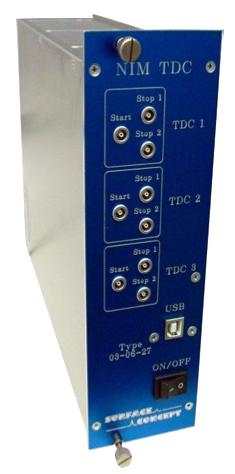
\includegraphics[height=0.25\textheight, width=\textwidth, keepaspectratio]{figures/NIM_TDC.png}
        \caption{Time to Digital Converter (TDC)}
        \label{fig:TDC}
    \end{subfigure}
    \hfill	
    \begin{subfigure}[t]{0.25\textwidth}
        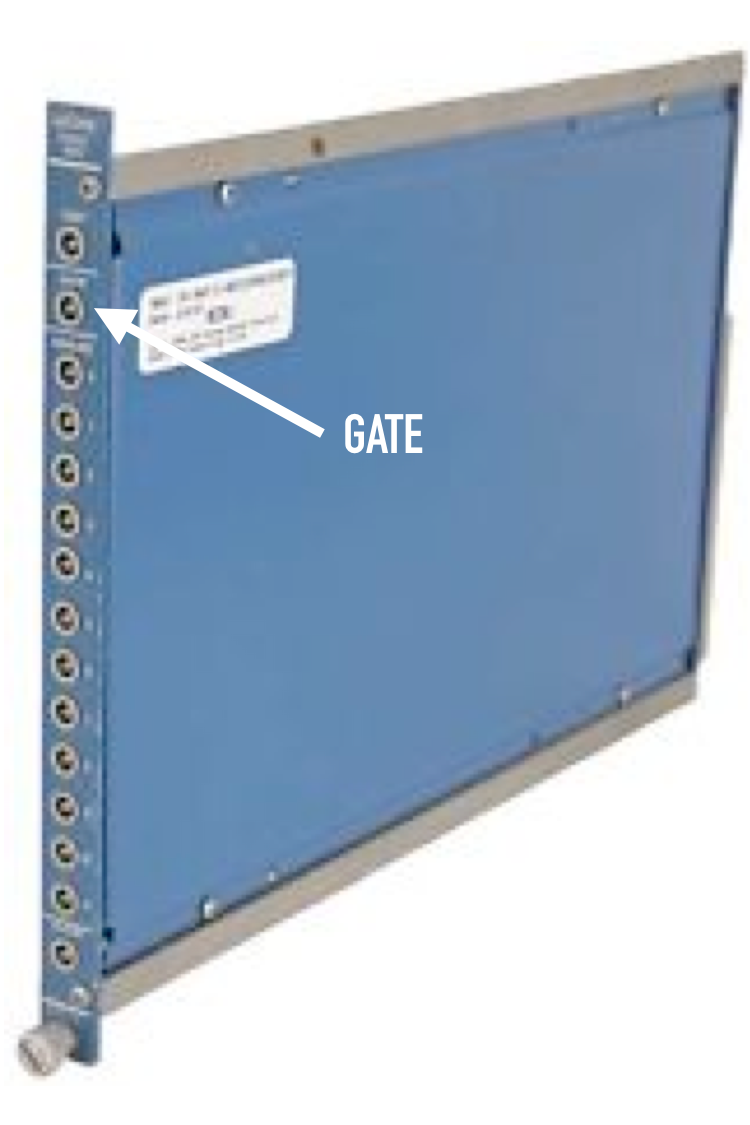
\includegraphics[height=0.25\textheight, width=\textwidth, keepaspectratio]{figures/gate.png}
        \caption{Analogue to Digital Converter (ADC)}
        \label{fig:}
    \end{subfigure}    
    \hfill
    \begin{subfigure}[t]{0.45\textwidth}
        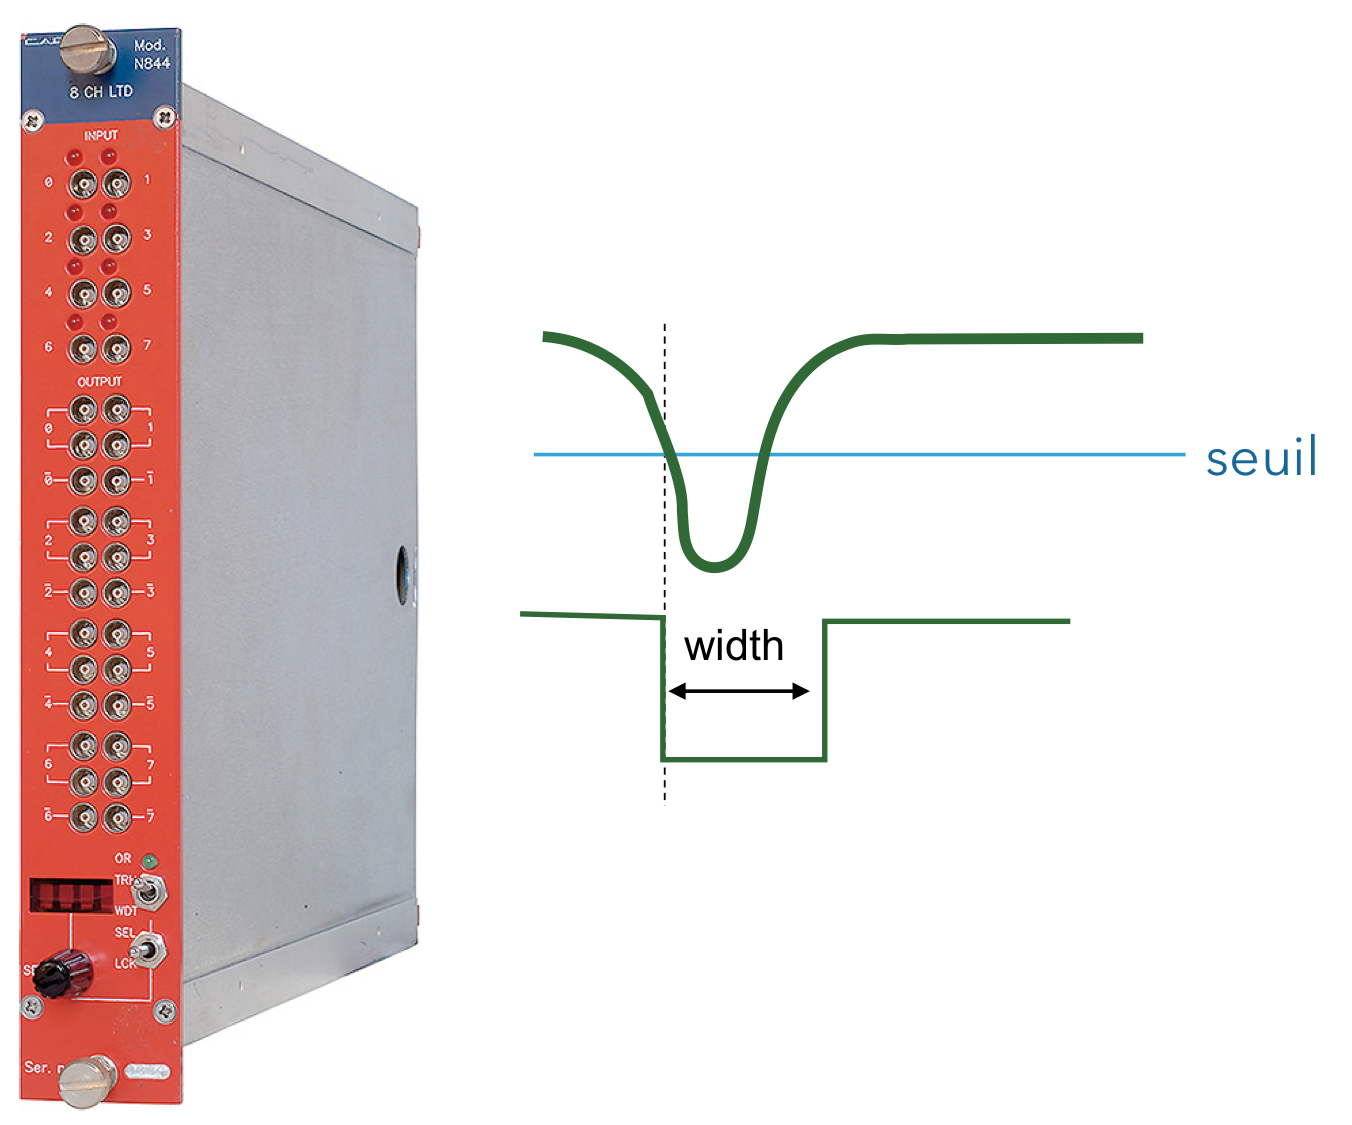
\includegraphics[height=0.3\textheight, width=\textwidth, keepaspectratio]{figures/Discriminateur.png}
        \caption{Discriminateur}
        \label{fig:discriminator}
    \end{subfigure}

	\vspace{1cm}    
    \begin{subfigure}[t]{0.45\textwidth}
        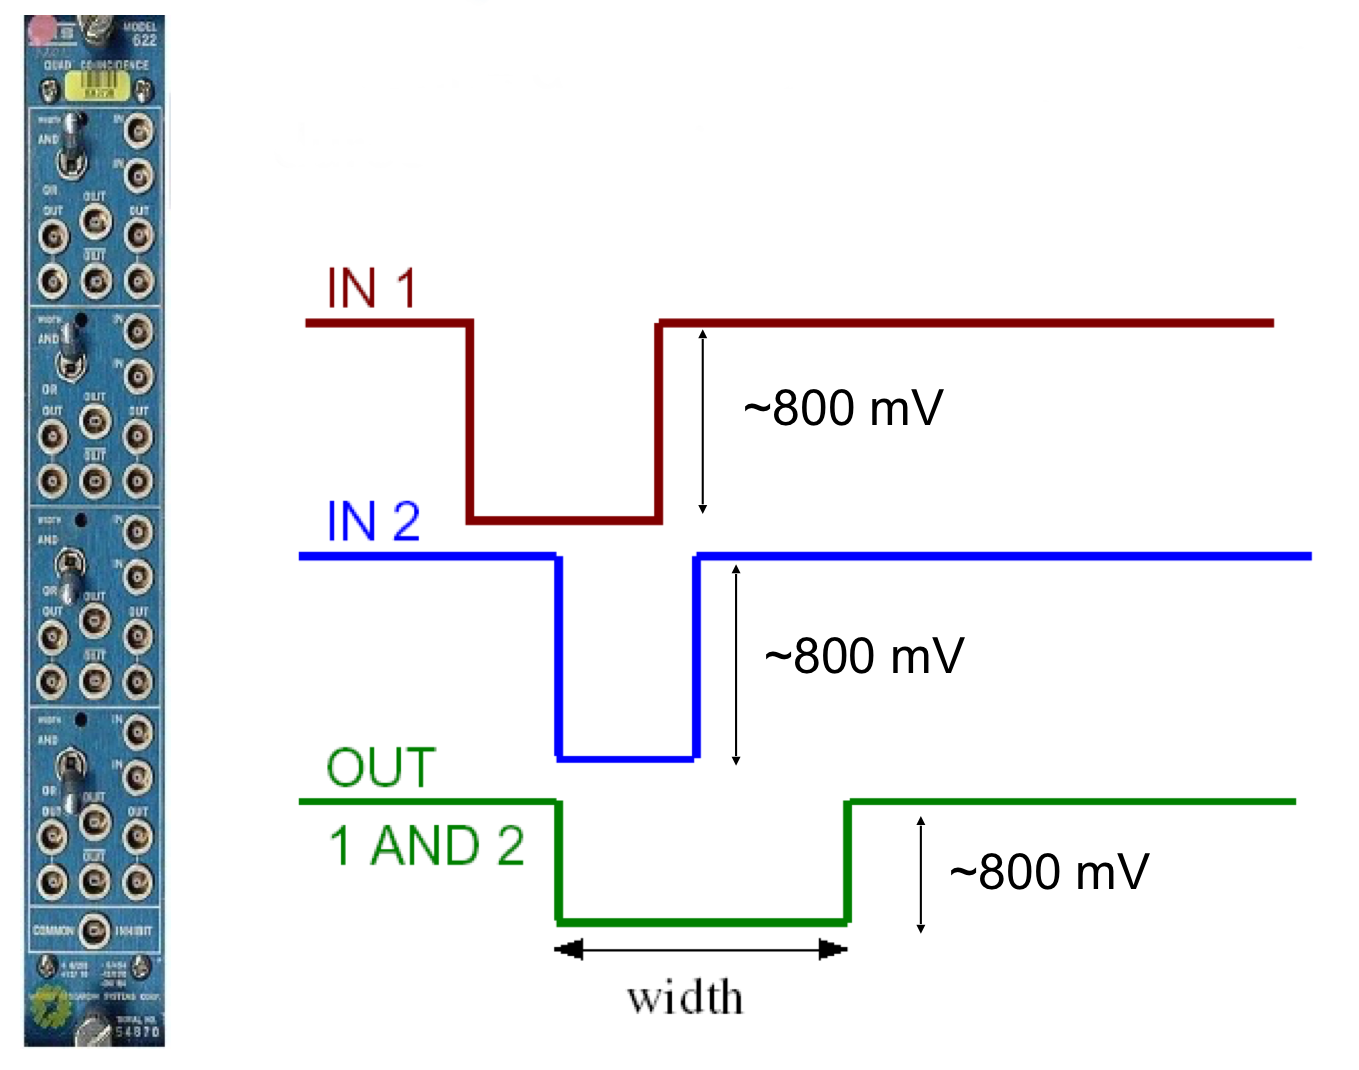
\includegraphics[height=0.3\textheight, width=\textwidth, keepaspectratio]{figures/UniteDeCoincidence_crop.png}
        \caption{Unit{\'e} de co{\"i}ncidence}
        \label{fig:coincidence}
    \end{subfigure}
    \hfill
    \begin{subfigure}[t]{0.45\textwidth}
        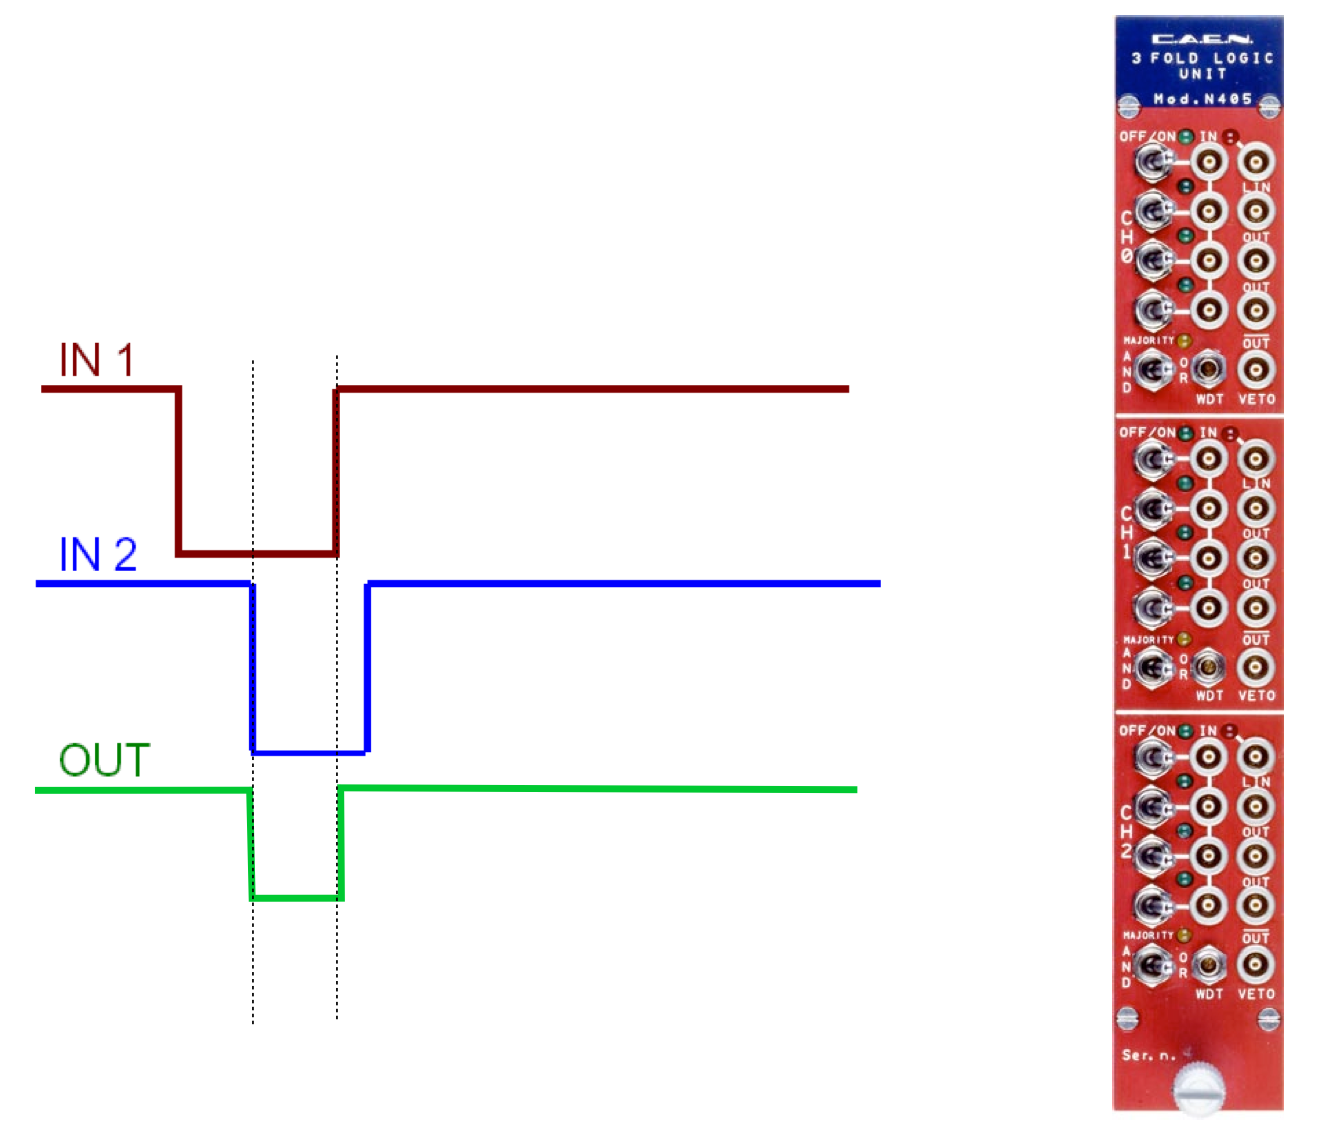
\includegraphics[height=0.3\textheight, width=\textwidth, keepaspectratio]{figures/UniteLogiqueProgrammable.png}
        \caption{Unit{\'e} logique programmable}
        \label{fig:programmable}
    \end{subfigure}
    \caption{Appareils utilis{\'e}s dans les dispositifs.}
    \label{fig:devices}
\end{figure}

\textbf{Fan-in-fan-out (FIFO)} [figure  \ref{fig:fifo}] :\\
Cette unité permet de dédoubler le signal. Il en existe 2 types:
\begin{itemize}
\item Logic FIFO : sort un signal logique
\item Linear FIFO : sort un signal analogique\\
\end{itemize}

\textbf{Unité de délai} [figure \ref{fig:delay}] :\\
Cette unité sort un signal identique au signal d'entrée en lui ajoutant un délai.\\

\textbf{Time to Digital Converter (TDC)} [figure \ref{fig:}] :\\
Ce module permet de reconnaître un évènement et de fournir une représentation digital du moment auquel il est survenu. Ces unités sont communément utilisées pour mesurer un interval de temps et le convertir en une sortie digitale.\\

\textbf{Analogue to Digital Converter (ADC)} [figure \ref{fig:}] :\\
Ce module mesure une charge ou une différence de potentiel. 
La charge, présentée à l’entrée pendant un intervalle de temps fixé par un signal logique fourni à l’ADC (gate), est accumulée sur un condensateur. Dans un second temps, on laisse le condensateur se décharger au travers d’un circuit RC et on compte le temps nécessaire à cette décharge. Pour se faire, on compte les impulsions d’un oscillateur, au moyen d’une échelle de comptage (scaler). Chaque module possède 12 entrées.\\

\textbf{Discriminateur} [figure \ref{fig:discriminator}] :\\
Donne un signal logique si le signal d'entée atteint un certain seuil. Pour une unité de logique standard NIM, le "vrai" est fixé à -800 mV. Le seuil et la largeur du signal analogique peuvent être modifié.\\

\textbf{Unité de coïncidence} [figure \ref{fig:coincidence}] :\\
Cette unité donne un signal logique lorsqu'on a un signal coïncident des entrées. On peut sélectionner la durée du signal sortant.\\

\textbf{Unité logique programmable} [figure  \ref{fig:programmable}]  :\\
Ce module permet d'effectuer des sorties selon une table de logique programmée au préalable. Il possède 4 entrées ainsi que 4 sorties, ce qui permet d'obtenir 16 lignes de logique. La durée de la sortie est déterminée par le temps durant lequel on a coïncidence. \\